% ===============================================================
% =							Related Work 						=
% ===============================================================
\chapter{Results and Evaluation}
\label{cha:results}

To experiment the results of our tool, we took various approaches as for testing. In this chapter we describe the methods and results of the tests and inquiries on a group of users.

\section{Algorithm Comparison}

Since we decided to use modified version of some algorithms to try and use them in a real-time environment, it made sense to compare our results with ones obtained from the original algorithms. 
One the algorithms we used that was partially implemented, was the object segmentation (Section \ref{sub:segmentation}). For this algorithm we opted for not using Grabcut \cite{rother2004grabcut} to refine the results since the saliency map already gave a good indication of what was the object in a scenario.  To compare with the original algorithm, we used the same dataset as the author and compared the resulting segmentation masks.

From a subset of 500 images from the original dataset, we ran our implementation and could conclude that for almost all the images, a significant part of the main subject in the photo was always detected. Since we decided no to use Grabcut, our results could not be refined and therefore our segmentation mask would have allot of unfilled areas that were still considered as part of the subject. In other cases, the saliency map that we implemented completely failed. Some of the reasons for this to fail was the lack of contrast of the subject in comparison to the background or because the background had higher contrast. Another thing that highly influences the results is the brightness because bright areas were more likely to be chosen as part of the subject.

As referred in Section \ref{sub:segmentation}, our segmentation mask was based on pixels that were considered as foreground while all other were background. In an attempt to fill the areas that were not considered foreground and still belonged to the subject, we considered all pixels as foreground since they were inside of a bounding area. We also did a comparison of the method with the original algorithm using the same subset of images. 
For the tested images, it fulfilled its purpose. However, in most images it ruins the results because many background elements are then added to the mask. Some of the results can be seen and compared in Annex \ref{app:seg_results}.


Another algorithm we tested, was the colour template detection. For this feature we implemented a more simple algorithm instead of simplifying the original one. However, \citeauthor{cohen2006color} \cite{cohen2006color} didn't describe any methods of evaluation for this algorithm. We then used a couple of images that showed results and compared the results of our own algorithm. In Annex \ref{app:temp_results} it is possible to observe some images used by the author and compare the results obtained from the original algorithm with our results. From what we could conclude, our results were not to far from the expected and still give a good indication if the colour is using a monochromatic or complementary template, and what are the most salient colours.

\section{Algorithm Execution Time}

Having the purpose of displaying information in real-time, we considered that the execution times of each algorithm should be taken into account. Algorithms with a slow performance are less likely to be useful in a real-time scenario and might even ruin the experience of the user. With that in mind, we did performance tests over each feature to understand its reliability in real-time processing.


\subsection{Testing tool}
These times were taken by generating log files that contain trace information to analyse. We used the Android's \emph{Debug} class to call the methods \emph{startMethodTracing()} and \emph{stopMethodTracing()}, to start and stop logging of trace information to disk. This option is very precise because we can specify exactly where to start and stop logging trace data in your code. For all tests we started the profile in the moment that the application receives a frame from the device's camera, and stopped right after processing that frame and refresh the view of the current feature \cite{SDK}.

After generating the log files, we used a tool called \emph{dmtracedump} to generate a graphical call-stack diagram from the trace log files. Figure \ref{fig:trace_ex} illustrates an example of the generated diagram from a trace file. 
In this tree diagram each call is represented as a node, and shows the call flow (from parent node to child node) using arrows. For each node, \emph{dmtracedump} shows \emph{<ref> callname (<inc-ms>, <exc-ms>,<numcalls>)}, where

\begin{itemize}
\item \emph{<ref>} - Call reference number, as used in trace logs,
\item \emph{<inc-ms>} - Inclusive elapsed time (milliseconds spent in method, including all child methods),
\item \emph{<exc-ms>} - Exclusive elapsed time (milliseconds spent in method, not including any child methods),
\item \emph{<numcalls>} - Number of calls.
\end{itemize}

\begin{figure}[htb]
	\centering
	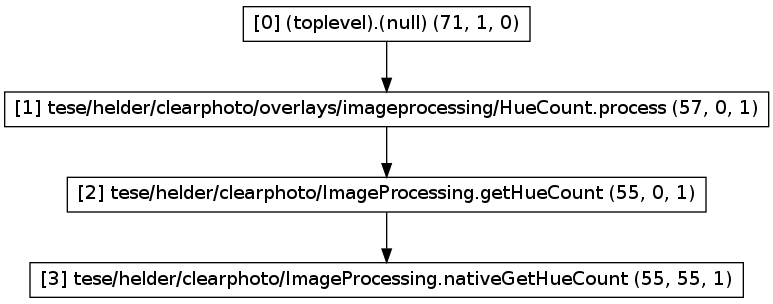
\includegraphics[width=\textwidth]{interface/trace.png}
	\caption{Graphical diagram generated from a trace log file.}
	\label{fig:trace_ex}
\end{figure}

Using the trace log file and these diagrams, we were able to get the amount of milliseconds spent in a method and any method called by it (\emph{<inc-ms>}), and the total time it took to perform the computation from the start to finish.
For each feature we took 10 samples and ignored the lowest and highest value to then calculate the average time and standard deviation for the total amount of time it took to perform the trace and the time spent in the method that processed the data. This way we expect to obtain relevant information about the time spent processing the frame and refreshing the view of each feature.

\subsection{Results}

All the times taken are in Annex \ref{app:exec_times} represented by a table with the time of each sample and the average of total time spent.
Some of these features where tested under different conditions or parameters to understand the difference in performance. For example, the saturation detection (Table \ref{tab:sat}) was tested in scenarios where the detector successfully indicated low saturation and in scenarios where it failed. We could conclude by the samples taken that the detector performs better when it fails to detect a low saturation environment. This is due to the extra computational effort that the device has to make to convert the frame into grayscale to display on the viewfinder. However the algorithm is not that heavy and it still performs quite well, disregarding the visual cue that can easily be replaced by a more appropriate one.

Another feature that we experimented in different scenarios was the face detection (Table \ref{tab:face}). We experimented detecting one or three faces as well as using the suggestions for boosting the composition. As we can conclude from the results, there weren't any significant changes from each one the scenarios. As expected, the most costly computation was the detection of a face in a frame. In comparison, the calculation of the suggestion to improve the composition is neglectable.

The detection of main lines is dependent of a threshold, therefore we sampled the algorithm with different thresholds. The threshold values tested were 160, 100 and 40 as lower thresholds detect more lines. As we can conclude from Table \ref{tab:major_lines}, for all thresholds the computational effort was similar regardless of the threshold.

We also implemented three algorithms to calculate the simplicity on an image, therefore, the performance of each one was tested individually (Table \ref{tab:simplicity}). We could conclude that the fastest method was the second method described by \citeauthor{kaoautomatic} \cite{kaoautomatic}. However, as discussed in Section \ref{subsub:simp_disc}, this is the least reliable method comparing to the other two. On the other end, the first method \cite{luo2008photo} and the third method \cite{ke2006design} tested are slower but more reliable. Being approximately 50ms slower, any of these methods is a good option.

From the remaining features, the features that performed better were the histograms calculation, detection of templates and scoring based on the \emph{Hue} channel. For the sampled tests, all these features performed in 50~150ms which can be translated into 6~20 frames-per-second, where the colour histogram in the \emph{Hue} channel and colour template detection had the slowest times. 

On the other end, the slowest feature were the object segmentation, the image balance and the detection of the horizon line, with average times of approximately 240ms, 600ms and 2700ms, respectively. Being more complex algorithms, these results were expected. However, detecting the image balance and the horizon line, are algorithms too expensive to be used on a real-time scenario. Object segmentation and horizon line detection are algorithms that give important visual feedback since they work as an overlay over the real frame, however both algorithms perform poorly.

 
\section{Usability Testing}